\section{The Chainsewing Attack}
We  will now describe an explicit attack against the NIPoPoW suffix proof construction under velvet fork. As already argued, since the protocol is implemented under velvet fork, any thorny block be accepted as valid. Taking advantage of such blocks in the chain, the adversary could produce suffix proofs containing an arbitrary number of blocks belonging in several fork chains. The attack is described in detail in the following.

Assume that chain $\chain_B$ was adopted by an honest player B and chain $\chain_\mathcal{A}$, a fork of $\chain_B$ at some point, maintained by adversary $\mathcal{A}$. Assume that the adversary wants to produce a suffix  proof in order to attack a light client to have him adopt a chain which contains blocks of $\chain_\mathcal{A}$. In order to achieve this, the adversary needs to include a greater amount of total proof-of-work in her suffix proof, $\pi_\mathcal{A}$, in comparison to that included in the honest player's proof, $\pi_B$, so as to achieve $\pi_\mathcal{A} \geq_m \pi_B$. For this she produces some thorny blocks in chains $\chain_\mathcal{A}$ and $\chain_B$ which will allow her to claim blocks of chain $\chain_B$ as if they were of chain $\chain_\mathcal{A}$ in her suffix proof.

The general form of this attack for an adversary sewing blocks to one forked chain is illustrated in Figure \ref{fig:generic_attack}. Dashed arrows represent interlink pointers of some level $\mu_\mathcal{A}$. Starting from a thorny block in the adversary's forked chain and following the interlink pointers, a chain is formed which consists the adversary's suffix proof. Blocks of both chains are included in this proof and a verifier could not distinguish the non-smooth pointers participating in this proof chain and, as a result, would consider it a valid proof.

\begin{figure}[h]
	\begin{center}
		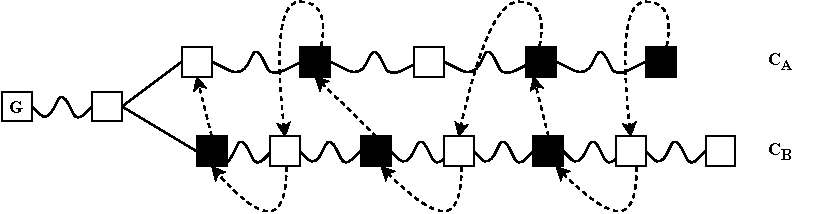
\includegraphics[scale=0.63
		]{figures/generic_chainsewing_attack.pdf}
	\end{center}
	\caption{\textit{Generic Chainsewing Attack. $\chain_B$ is the chain of an honest 	player and $\chain_\mathcal{A}$ the adversary's chain. Adversarially generated blocks are 	colored black. Dashed arrows represent interlink pointers included in the 	adversary's suffix proof. Wavy lines imply one or more blocks.}}
	\label{fig:generic_attack}
\end{figure}

As the generic attack scheme may seem a bit complicated we will now describe a more specific attack case. Consider that the adversary acts as described below. Assume that the adversary chooses to attack at some level $\mu_\mathcal{A}$. As shown in Figure \ref{fig:attack} she first generates a superblock $b'$ in her forked chain $\chain_\mathcal{A}$ and a thorny block $a'$ in the honest chain $\chain_B$ which points to $b'$. As argued earlier, block $a'$ will be accepted as valid in the honest chain $\chain_B$ despite the invalid interlink pointers. After that, the adversary may mine on chain $\chain_\mathcal{A}$ or $\chain_B$, or not mine at all. At some point she produces a thorny block $a$ in $\chain_\mathcal{A}$ pointing to a block $b$ of $\chain_B$. Because of the way blocks are generated by updated honest miners there will be successive interlink pointers leading from block $b$ to block $a'$. Thus following the interlink pointers a chain is formulated which connects $\chain_\mathcal{A}$ blocks $a$ and $b'$ and contains an arbitrarily
large part of the honest player's chain $\chain_B$.

At this point the adversary will produce a suffix proof for chain $\chain_\mathcal{A}$ containing the subchain $\chain\{ab\} \cup \chain\{b{:}a'\} \cup \chain\{a'{:}b'\}$. Notice that following the interlink pointers constructed in such a way, a light client perceives $\chain\{ab\} \cup \chain\{b{:}a'\} \cup \chain\{a'{:}b'\}$  as a valid chain.

\begin{figure}[h!]
	\begin{center}
		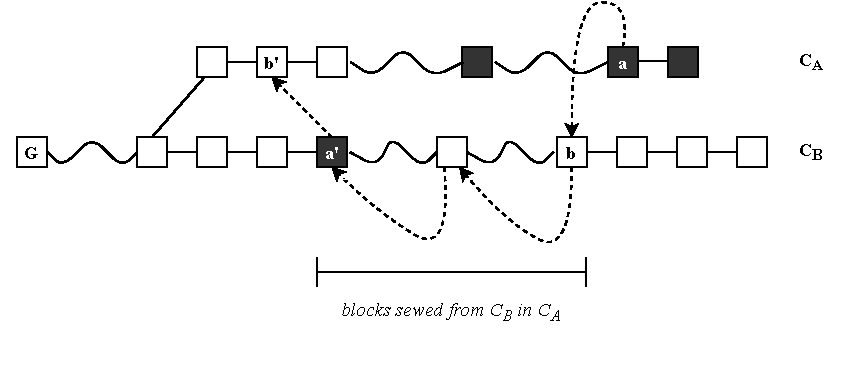
\includegraphics[scale=0.63]{figures/chainsewing_attack.pdf}
	\end{center}
	\caption{\textit{
		Chainsewing Attack. $\chain_B$ represents the chain of an honest 	player. $\chain_\mathcal{A}$ is an adversarial fork. Adversarially generated blocks are colored black. Dashed arrows represent	interlink pointers included in the adversary's suffix proof. Wavy lines imply one or more blocks. Firm lines imply the previousId 	relationship between two sequential blocks.}}
	\label{fig:attack}
\end{figure}

In this attack the adversary uses thorny blocks to ``sew`` portions of the chain adopted by an honest player to her own forked chain. This remark justifies the name given to the attack.

Note that in order to make this attack successful, the adversary has to produce only a few superblocks which let her arrogate an arbitrarily large number of blocks. Thus this attack is expected to succeed with overwhelming probability.

%@TODO
%Needs to be proven. It is not obvious that the attacker will succeed in high probability, since the most important adversarially generated blocks , $a$ and $a'$, set a limit to the adversarial blocks produced in parallel to the honest blocks of subchain $C\{ab\} \cup C\{b{:}a'\} \cup C\{a'{:}b'\}$ and can take part in the suffix proof.
